\chapter{Анализ предметной области} \label{chapt2}
\section{Типы индексов}
\subsubsection{B-Tree}
\begin{figure}[ht]
	\centering
	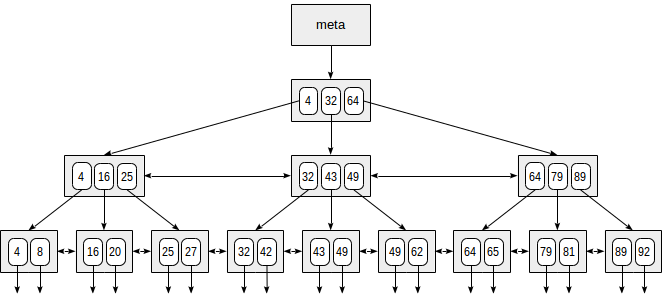
\includegraphics [scale=0.5] {btree}
	\caption{Схематичный пример индекса по одному полю с целочисленными ключами}
	\label{img:btree}
\end{figure}
Для хранения данных в отсортированном виде используется B-Tree. Чтобы примерно представить себе работу следует вспомнить обычное бинарное дерево (поиск по нему имеет логарифмическую скорость поиска элемента). Однако в данном случае всё устроено сложнее: дерево сбалансировано и сильно ветвистое --- каждый узел обычно имеет более двух потомков ~\ref{img:btree}.

Элементы данного дерева отсортированы по возрастанию.
Что позволяет эффективно выполнять поиск как отдельного значения,
так и интервала значений. Ситуация ухудшается, когда необходимо
делать поиск по нескольким измерениям. В этом случае мы можем ограничить
лишь одно измерение, поиск по другим будет производиться полным перебором.

Тем не менее для большинства задач B-дерево всё-таки является хорошим вариантом. B-Tree можно назвать самым популярным индексом, использующимся в большинстве современных СУБД как реляционных, так и нереляционных при этом абсолютно не важно,
где именно хранятся данные --- в памяти или на диске.
Существует много модификаций B-Tree: B+Tree (используется в CouchDB, MongoDB), SB-Tree (OrientDB), B*-Tree.

B-дерево было предложено ещё в 1970 году для эффективного поиска среди файлов~\cite{bayer2002organization}, с тех пор появилось большое количество эффективных и компактных реализаций этой структуры.
Такую популярность данная структура получила благодаря своей работе с памятью.
Если мы хотим прочитать какое-либо значение, то в память/кэш
помещается весь блок данных. Что существенно ускоряет скорость чтения,
если кроме этого потребуются и соседние значения. Однако это является
и недостатком этой структуры --- если требуется записать новое или
перезаписать существующее значение, будет обновлен весь блок.
Такие <<паразитные>> чтения в литературе,
посвящённой хранению на диске, называется read amplification,
а <<паразитные>> записи --- write amplification.
Формально, amplification factor, то есть коэффициент умножения,
вычисляется как отношение размера фактически прочитанных (или записанных) данных к реально необходимому (или измененному) размеру.
В случае B-дерева порядок этого коэффициента --- десятки и сотни.

\subsubsection{Hash}
Hash--индекс работает не с индексируемыми ключами, а с их хэшами. Идея хеширования состоит в том, чтобы значению любого типа данных сопоставить некоторую битовую последовательность фиксированной длины. Такое сопоставление называют хеш-функцией. Полученное значение можно использовать как индекс обычного массива, куда и складывать ссылки на строки таблицы.

Это следующий по популярности индекс. Главным недостатком является то, что в запросах поддерживается только операция равенства. Кроме того, возникают коллизии (когда одному хэшу соответствует несколько значений) и трудности с хранением null--значений.

В отличие от других вариантов хранится не само значение, а его хэш, что делает этот индекс компактным и быстрым.

\subsubsection{LSM-Tree}
Ещё одним типом дерева, наравне с B-Tree, предназначенным для хранения
данных является LSM-Tree --- \textit{Log-structured merge-tree}~\cite{lsmtree1996}.
В отличие от B-Tree, которое можно использовать
как для хранения в памяти, так и на диске, LSM-Tree предназначено
для хранения данных именно на диске. Разделение на части, хранящиеся
в памяти и на диске заложено в саму архитектуру данной структуры.
Все операции вставки делаются в L0 (уровень, хранящийся в оперативной памяти), как только место там заканчивается, данные начинают сбрасываться на диск (рис.~\ref{img:lsm_tree}).

Ещё одним ключевым отличием является то,
что в узлах дерева хранятся не сами данные, а операции с ними (рис.~\ref{img:lsm_tree_ops}).

\begin{figure}[ht]
	\centering
	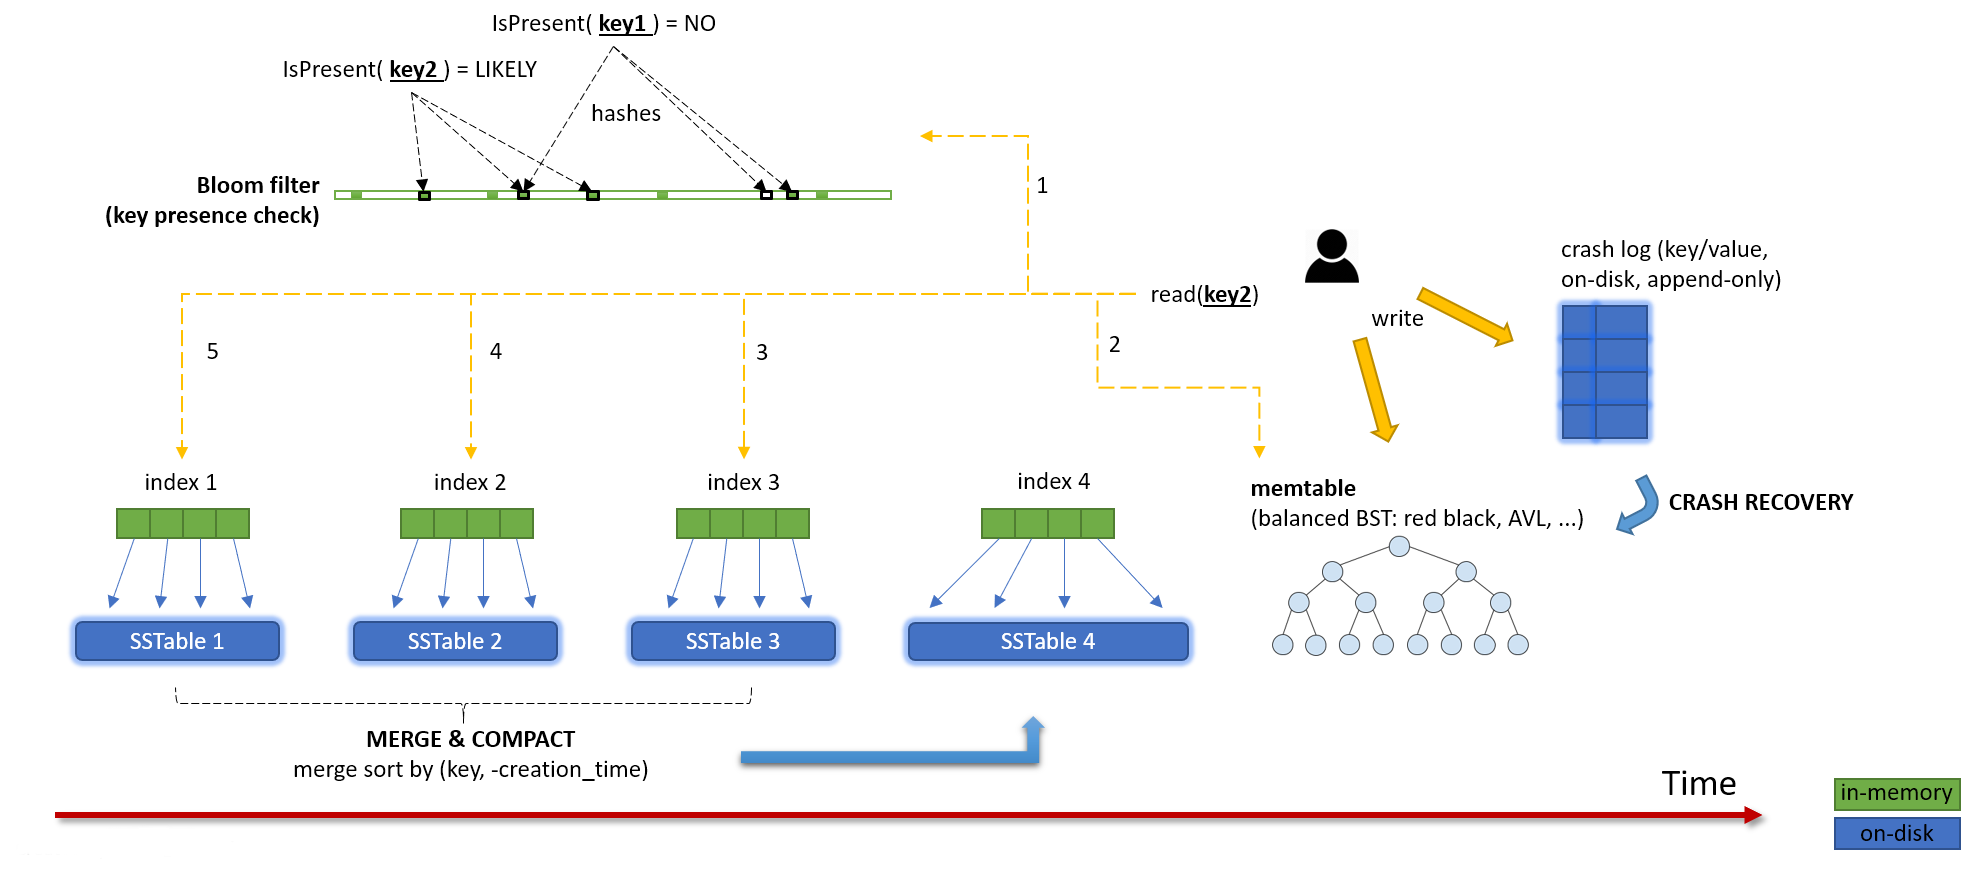
\includegraphics [scale=0.5] {lsm_tee.png}
	\caption{Схематическое представление LSM-Tree}
	\label{img:lsm_tree}
\end{figure}


\begin{figure}[ht]
	\centering
	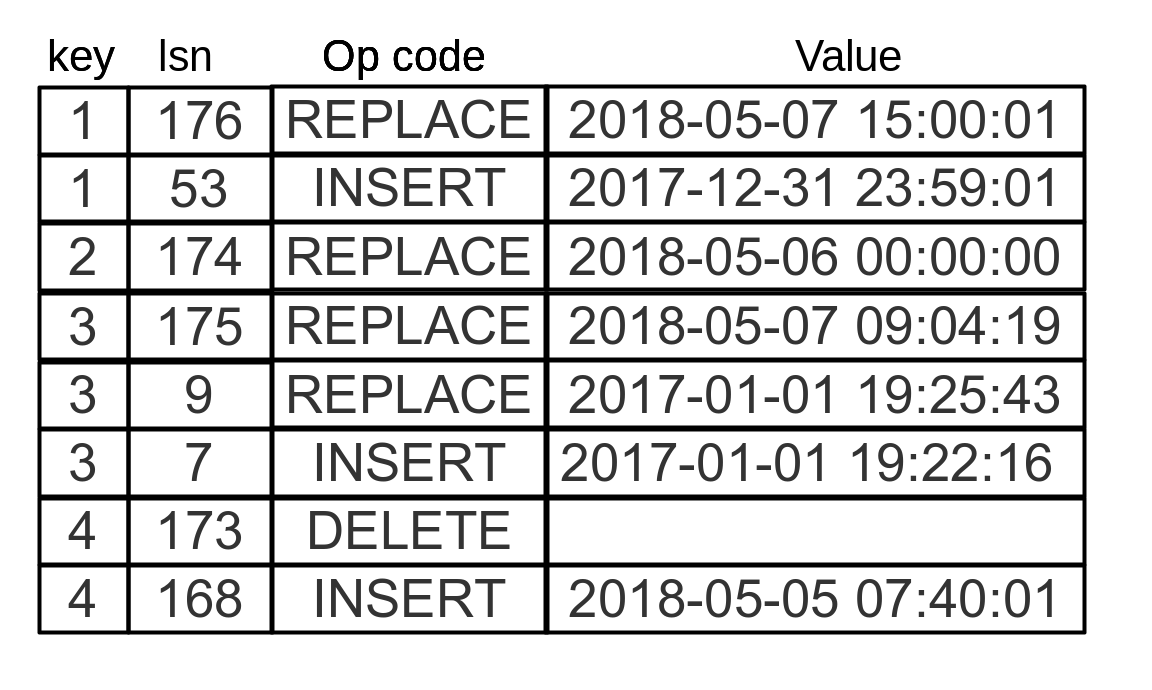
\includegraphics [scale=0.3] {lsm_tree_ops}
	\caption{Хранение операций над данными, а не самих данных}
	\label{img:lsm_tree_ops}
\end{figure}

LSM-деревья работают быстрее для частых вставок и редких чтений, в отличие от B-деревьев, иными словами write amplification LSM-деревьев
меньше, но read amplification выше. LSM-деревья стали довольно популярны
в последнее время, это связано с тем, что стоимость внешней памяти
стала меньше, при этом популярность приобретают SSD-диски,
обладающие более высокой скоростью чтения по сравнению с устаревающими
HDD-дисками.

\subsubsection{Inverted index}
Индекс, использующаяся для полнотекстового поиска. Содержит список всех уникальных слов и ссылки на документы, в которых эти слова встретились.

Полнотекстовые запросы выполняют лингвистический поиск в текстовых данных путем обработки слов и фраз в соответствии с правилами конкретного языка: разбиение на слова, отсекание окончаний, выбор однокоренных слов и т.д. Отдельными задачами при полнотекстовом поиске являются ранжирование результатов запроса и исключение ненужных слов.

Реализации полнотекстового поиска варьируются в различных СУБД. Инвертированный индекс используется в Microsoft SQL Server, MySQL, OrientDB и поисковом движке Elasticsearch.

Обобщением данного типа индекса является \textit{GIN} (Generalized Inverted Index),  реализованный в PostgreSQL.
Кроме полнотекстового поиска, является подходящим для индексирования массивов и JSON. Обобщенным он называется, потому что операция над индексируемым объектом задается отдельно в отличие от, например, B-Tree, где все операции сравнения уже заданы. В качестве операция могут использоваться такие как <<содержит>>, <<пересекается>>, <<содержится>>.

Количество текстовой информации, окружающей нас огромно: новости, книги, письма и т.д. Для индексирования содержимого этот тип индекса является подходящим. Однако работа с текстом не входит в поставленную задачу.

\subsection{Пространственные индексы}
Большинство современных СУБД имеют типы, предназначенные для работы с пространственными типами данных: точки, прямые, окружности и другие геометрические объекты. Для данных объектов используются свои стратегии индексирования.

Известными решениями является использование пространственной сетки (spatial grid), дерева квадрантов (quadtree) и R-Tree.

Данные индексы используются графовыми базами данных (Neo4j, AllegroGrath), однако существуют специальные дополнения и расширения для известных СУБД, но предназначенные для обработки исключительно пространственной информации --- PostGIS, Oracle Spatial, GeoAPI в Redis.

\subsubsection{R-Tree}
\begin{figure}[ht]
	\centering
	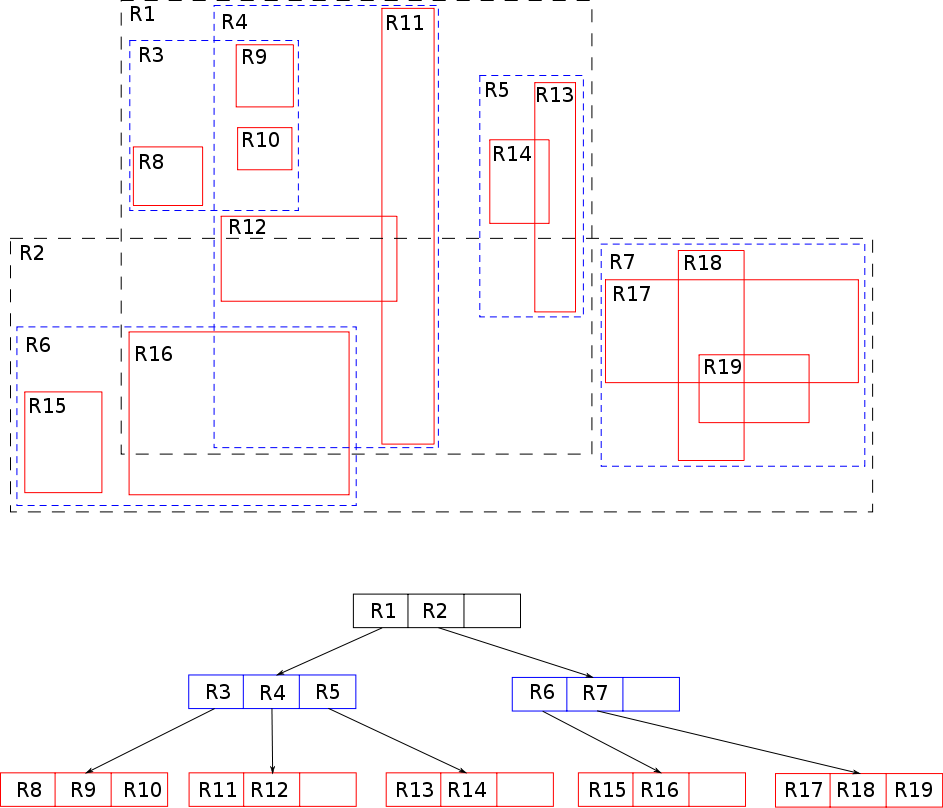
\includegraphics [scale=0.5] {rtree}
	\caption{Пример организации хранения данных в R-Tree}
	\label{img:rtree}
\end{figure}

Эта структура данных разбивает многомерное пространство на множество иерархически вложенных и, возможно, пересекающихся, прямоугольников и гиперкубов (для многомерных структур)~\ref{img:rtree}.

Подходит для поиска объектов в 2-3--мерном пространстве. Идея лежащая в основе индекса --- группировка объектов в зависимости от расстояния друг до друга. Это ускоряет поиск, однако происходит потеря точности, и возвращенный результат может не быть абсолютно точным.

Данный тип индекса поддерживается некоторыми движками СУБД MariaDB (SPATIAL INDEX), PostgreSQL (RTREE), Oracle.

Существует несколько модификаций R-Tree: R+-Tree, R*-Tree. Обобщением R-Tree является X-Tree, который позволяет индексировать данные произвольных размерностей.

Другое обобщение \textit{GiST (The Generalized Search Tree)} --- обобщенное дерево поиска. Реализовано в PostgreSQL и подобно GIN поддерживает индексирование произвольной информации (геоданные, тексты, изображения и т.д.) с использованием операций <<принадлежит>>, <<содержит>>, <<совпадает>>, <<соответствует>>.

\subsubsection{Z-order curve (Кривая Мортона)}
Индекс используемый для хранения многомерных данных в одномерной структуре. К каждому значению применяется преобразование Мортона, заключающееся в чередовании двоичных цифр координатных значений, полученный результат называется Z-последовательностью (Z-order curve). Для обработки одномерных данных используется обычное B-дерево.

\begin{figure}[ht]
	\centering
	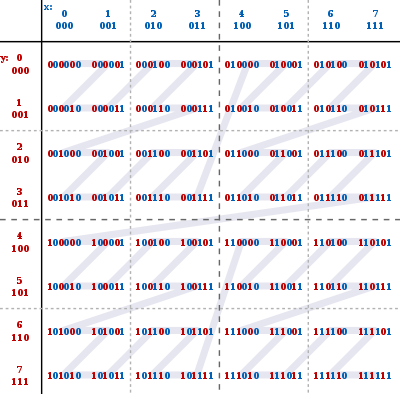
\includegraphics [scale=0.5] {zcurve2d}
	\caption{Построение Z-последовательности}
	\label{img:zcurve2d}
\end{figure}

Позволяет эффективно производить поиск по интервалам значений, однако часть возвращаемого результата может и не находиться в указанном интервале (рис.~\ref{img:zcurve2d_interval}), поэтому при запросе приходится применять дополнительные механизмы для фильтрации данных. Это накладывает некоторые ограничения на целесообразность применения данного индекса. Запросы должны быть.

\begin{itemize}
	\item \textbf{Часто задаваемыми}. Распространена практика, когда часть параметров запроса не задается, а остается открытой, однако в данном случае это может серьезно влиять на производительность.
	\item \textbf{<<Избирательным>>}. Границы, устанавливаемые при запросе должны исключать большие объемы данных. Для неравномерно распределенных логических значений пространство поиска может быть сильно увеличено.
\end{itemize}

\begin{figure}[ht]
	\centering
	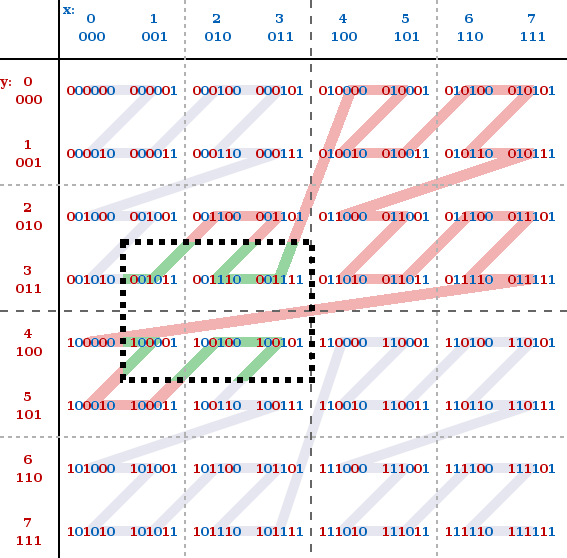
\includegraphics [scale=0.35] {zcurve2d_interval}
	\caption{Поиск значений в интервале}
	\label{img:zcurve2d_interval}
\end{figure}

При реализации Z-адрес рассматривается исключительно как битовая последовательность. Это значит, что единственное ограничение на тип ключа --- возможность упорядочивания при переходе к двоичному представлению. В итоге доступные типы ограничиваются не только целыми числами, но и числами с плавающей точкой, строками, временными метками...

Данный тип индексирование используется в TransBase\cite{ramsak2000integrating}, Accumulo, HBase \cite{nishimura2011md}, DynamoDB\cite{DynamoZorderP1, DynamoZorderP2}.

Стоит отметить, что данное преобразование не является единственным для отображения многомерных данных в одномерные. Могут использоваться кривые Гильберта или Пеано. Однако Z-последовательность гораздо проще для вычисления.

\subsection{Индексы c использованием машинного обучения}
Можно выделить несколько подходов, которые могут быть использованы для поиска информации и выделения закономерностей в больших массивах данных --- Latent Semantic Indexing (LSI) и Hidden Markov Model (HMM). Данные варианты хоть и являются интересными и полезными в некоторых сферах, но примеров их использования в каких--либо СУБД нет.

\section{Используемые индексы в различных СУБД}
\begin{tabular}{|c|c|{c}}
	\hline
	СУБД & Индексы\\
	\hline
	PostgreSQL & B-Tree, R-Tree, Hash, GiST,\\
	& SP-GiST, GIN, RUM, BRIN, Bloom  \\
	MySQL/MariaDB & B-Tree, Hash, R-Tree, Inverted Index  \\
	Oracle &  B-Tree, B-Tree--cluster,\\
	& Hash--cluster, Reverse key, Bitmap\\
	MongoDB & B-Tree, Geohash, Text index, Hash \\
	OrientDB & SB-Tree, Hash, Lucene Fulltext, Lucene Spatial \\
	MemSQL & SkipList, Hash, Columnstore \\ \hline
\end{tabular}

\section{Выбор платформы для разработки}

В качестве платформы, для которой будет реализован индекс на основе кривой Мортона
была выбрана СУБД Tarantool --- СУБД с открытым исходным кодом и
активно разрабатываемая в настоящее время.

Предлагаемое решение достаточно просто может быть встроено в существующую кодовую базу ---
около 400 тысяч строк на языке C и 200 тысяч строк на языке Lua.

Основные особенности СУБД Tarantool:

\begin{itemize}
	\item Удовлетворение принципу ACID
	\item Наличие двух движков для хранения данных на диске (vinyl) и в оперативной памяти (memtx) 
	\item Хранение данных в формате MessagePack
	\item Обработка транзакций в одном потоке
	\item Не только база данных, но и сервер приложений
\end{itemize}

Реализовываемый индекс будет работать с движком Memtx ---
все данные будут хранится в оперативной памяти.
Часть уже существующих решений может быть переиспользована, например,
B+*-Tree (BPS, в терминологии Tarantool).

В СУБД Tarantool достаточно необычная система типов.
При работе как с сервером приложений пользователь использует язык программирования
Lua 5.1 (LuaJIT 2.1 beta 2) и его типы: "string", "number" (double-precision floating-point),
"boolean", "table" (ассоциативный массив), "nil" (отсутствие значения),
а так же пользовательские типы данных, представленные типами "userdata" и "cdata".

Уровнем ниже находится MessagePack, обладающий большим количеством типов,
более близким к представленным в других языках программирования ---
unsigned int, signed int, float, double, \ldots С этим уровнем также взаимодействуют
коннекторы, позволяющие внешним системам работать с данными.

Ещё ниже следует система типов Tarantool, обладающая
типами которые могут сочетать в себе сразу несколько MessagePack типов, например,
"number" --- double для нецелых чисел, signed integer для отрицательных целых чисел
и unsigned integer для положительных чисел.

При реализации необходимо будет решить несколько инженерных задач:
\begin{itemize}
	\item Разработка пользовательского интерфейса для работы с индексом
	\item Встраивание решения в существующую кодовую базу
	\item Адаптация решения под существующую систему типов
\end{itemize}

Элементарной единицей является кортеж (tuple), аналог строки в
реляционных базах данных. Однако в отличие от реляционных БД
кортеж может иметь произвольную длину и содержать произвольные типы.
Строгая типизация требуется только для индексируемых полей.
